156. \begin{figure}[ht!]
\center{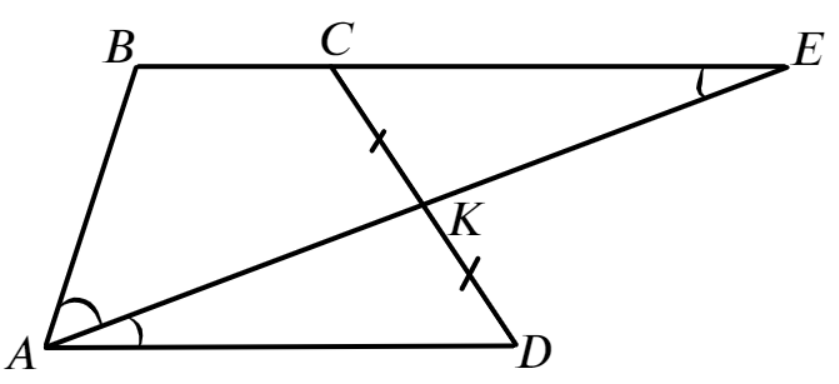
\includegraphics[scale=0.35]{g8-156.png}}
\end{figure}\\
Продлим $AK$ до пересечения с продолжением $BC$ в точке $E.$ Так как $AK$ является биссектрисой $\angle A,\ \angle BAE=\angle KAD.$ Углы $KAD$ и $KEC$ являются накрест лежащими, поэтому $\angle KEC=\angle KAD=\angle BAE$ и треугольник $ABE$ является равнобедренным, $AB=BE=BC+CE.$ В треугольниках $ADK$ и $KCE:\ DK=KC,\ \angle AKD=\angle CKE\ (\text{вертикальные})$ и $\angle ADK=\angle KCE$ (накрест лежащие), значит эти треугольники равны по второму признаку и $CE=AD.$ Таким образом, $AB=BC+CE=BC+AD=4+10=14.$\\
